%% Prezentacja na seminarium dyplomowe (ok. 10 minut). Osobny cel kompilacji:
%% pdflatex presentation.tex   (CI: .github/workflows/build-thesis.yml)
%% Zdjęcia: figures/prezentacja/ (kopie pomniejszone; źródła w komentarzach).
\documentclass[aspectratio=169, 11pt]{beamer}

\usepackage[T1]{fontenc}
\usepackage[utf8]{inputenc}
\usepackage{lmodern}
\usepackage[polish]{babel}
\usepackage{tikz}
\usetikzlibrary{positioning, arrows.meta}

\graphicspath{{figures/prezentacja/}}

\usetheme{default}
\usecolortheme{default}
\setbeamercolor{structure}{fg=blue!60!black}
\setbeamercolor{frametitle}{fg=blue!60!black}
\setbeamertemplate{navigation symbols}{}
\setbeamertemplate{itemize items}[circle]
\setbeamerfont{frametitle}{size=\Large, series=\bfseries}

%% Dane pracy: te same, co w main.tex
\newcommand{\stTytulPL}{Projekt i realizacja energooszczędnego budzika z bezprzewodową konfiguracją oraz radiową synchronizacją czasu DCF-77}
\newcommand{\stAutor}{Mikołaj Wójcicki}
\newcommand{\stOpiekun}{dr inż. Jarosław Emilianowicz}
\newcommand{\stKierunek}{Teleinformatyka}
\newcommand{\stSpecjalnosc}{Utrzymanie sieci teleinformatycznych}

\title[Energooszczędny budzik]{\stTytulPL}
\author{\stAutor}
\institute{Kierunek: \stKierunek\\Specjalność: \stSpecjalnosc\\Opiekun: \stOpiekun}
\date{Seminarium Praca Dyplomowa, 2026}

\begin{document}

%% 1. Tytuł
\begin{frame}[plain]
  \titlepage
\end{frame}

%% 2. Problem i cel
\begin{frame}{Po co budzik, skoro jest telefon?}
  \begin{itemize}
    \item Telefon w sypialni to powiadomienia i ekran zamiast snu.
    \item Cel: budzik na baterii, który sam trzyma dokładny czas i ma osobny harmonogram na każdy dzień tygodnia.
    \item Budzik wyłącza się dopiero po ruchu (potrząśnięcie, pajacyki), więc nie da się go zdrzemnąć.
  \end{itemize}
\end{frame}

%% 3. Wymagania
\begin{frame}{Wymagania}
  \begin{itemize}
    \item \textbf{Czas:} godzina, minuty, sekundy, dzień tygodnia; korekta sygnałem radiowym DCF-77.
    \item \textbf{Alarmy:} inna godzina dla każdego dnia, włączanie i wyłączanie osobno, sygnał dźwiękowy.
    \item \textbf{Energia:} zasilanie z akumulatora Li-Po, ładowanie przez USB-C, jak najmniejszy pobór prądu.
    \item \textbf{Konfiguracja:} Bluetooth Low Energy i strona WWW, bez Wi-Fi.
  \end{itemize}
\end{frame}

%% 4. Architektura (rysunek w TikZ, bez zewnętrznego pliku)
\begin{frame}{Architektura}
  \centering
  \begin{tikzpicture}[
      blk/.style={draw, rounded corners, minimum width=3.1cm, minimum height=0.9cm, align=center, font=\small},
      mcu/.style={blk, fill=blue!10, minimum width=3.8cm, minimum height=1.6cm},
      >=Stealth]
    \node[mcu] (mcu) {nRF52832\\(moduł MDBT42Q)\\tryb uśpienia, RTC};
    \node[blk, left=1.4cm of mcu, yshift=1.2cm]  (dcf) {odbiornik DCF-77};
    \node[blk, left=1.4cm of mcu, yshift=-0.0cm] (acc) {akcelerometr LIS3DH};
    \node[blk, left=1.4cm of mcu, yshift=-1.2cm] (buz) {buzzer};
    \node[blk, right=1.4cm of mcu, yshift=1.2cm]  (epd) {e-papier 2,13''};
    \node[blk, right=1.4cm of mcu, yshift=0cm]    (btn) {przyciski};
    \node[blk, right=1.4cm of mcu, yshift=-1.2cm] (ble) {BLE $\to$ strona WWW};
    \node[blk, below=1.3cm of mcu, xshift=-2.6cm, minimum width=2.9cm] (chg) {ładowarka MCP73831};
    \node[blk, below=1.3cm of mcu, xshift=2.6cm,  minimum width=2.9cm] (bat) {Li-Po + USB-C};
    \draw[->] (dcf) -- (mcu);
    \draw[<->] (acc) -- (mcu);
    \draw[<-] (buz) -- (mcu);
    \draw[<-] (epd) -- (mcu);
    \draw[->] (btn) -- (mcu);
    \draw[<->] (ble) -- (mcu);
    \draw[->] (bat) -- (chg);
  \end{tikzpicture}
\end{frame}

%% 5. Prototyp
\begin{frame}{Prototyp sprzętowy}
  \begin{columns}[c]
    \begin{column}{0.30\textwidth}
      \centering
      %% źródło: notes/media/2026-10-25_deep-sleep_ppk2-C.jpg
      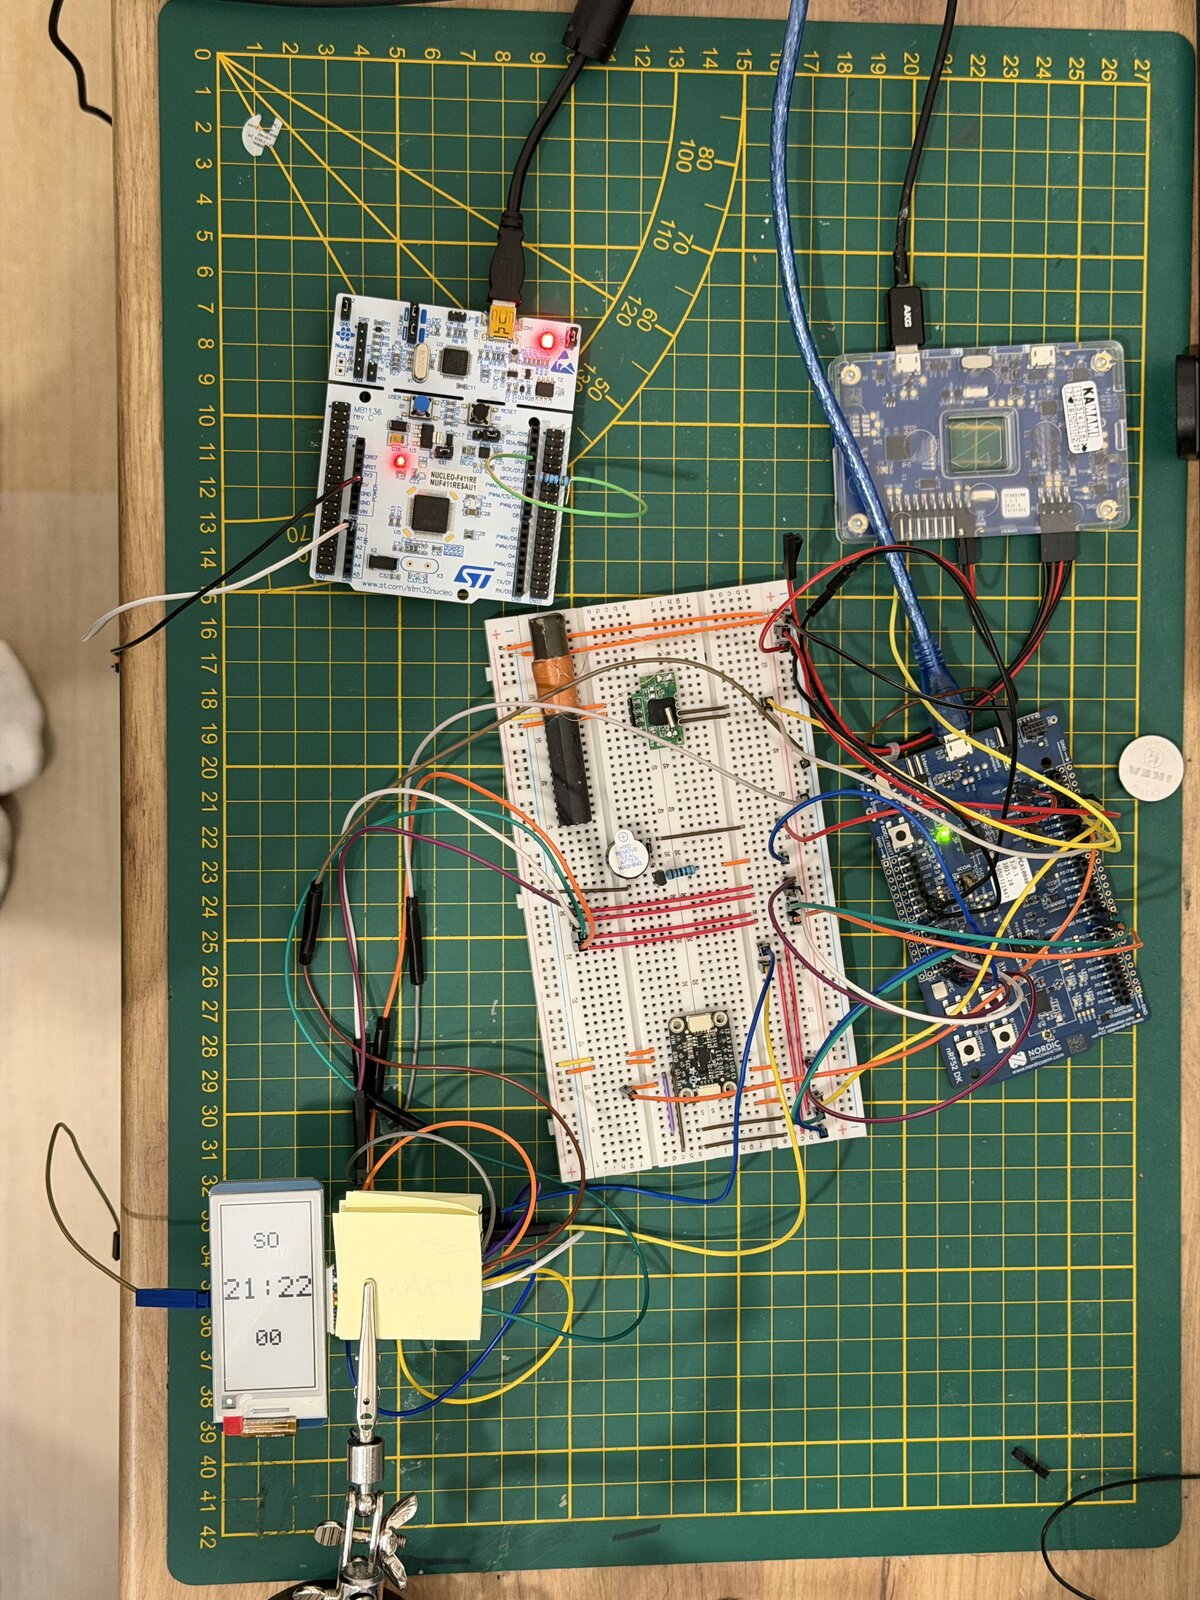
\includegraphics[height=0.66\textheight]{bench-breadboard.jpg}
    \end{column}
    \begin{column}{0.30\textwidth}
      \centering
      %% źródło: temp-resources, tył modułu e-papieru (zdjęcie z telefonu)
      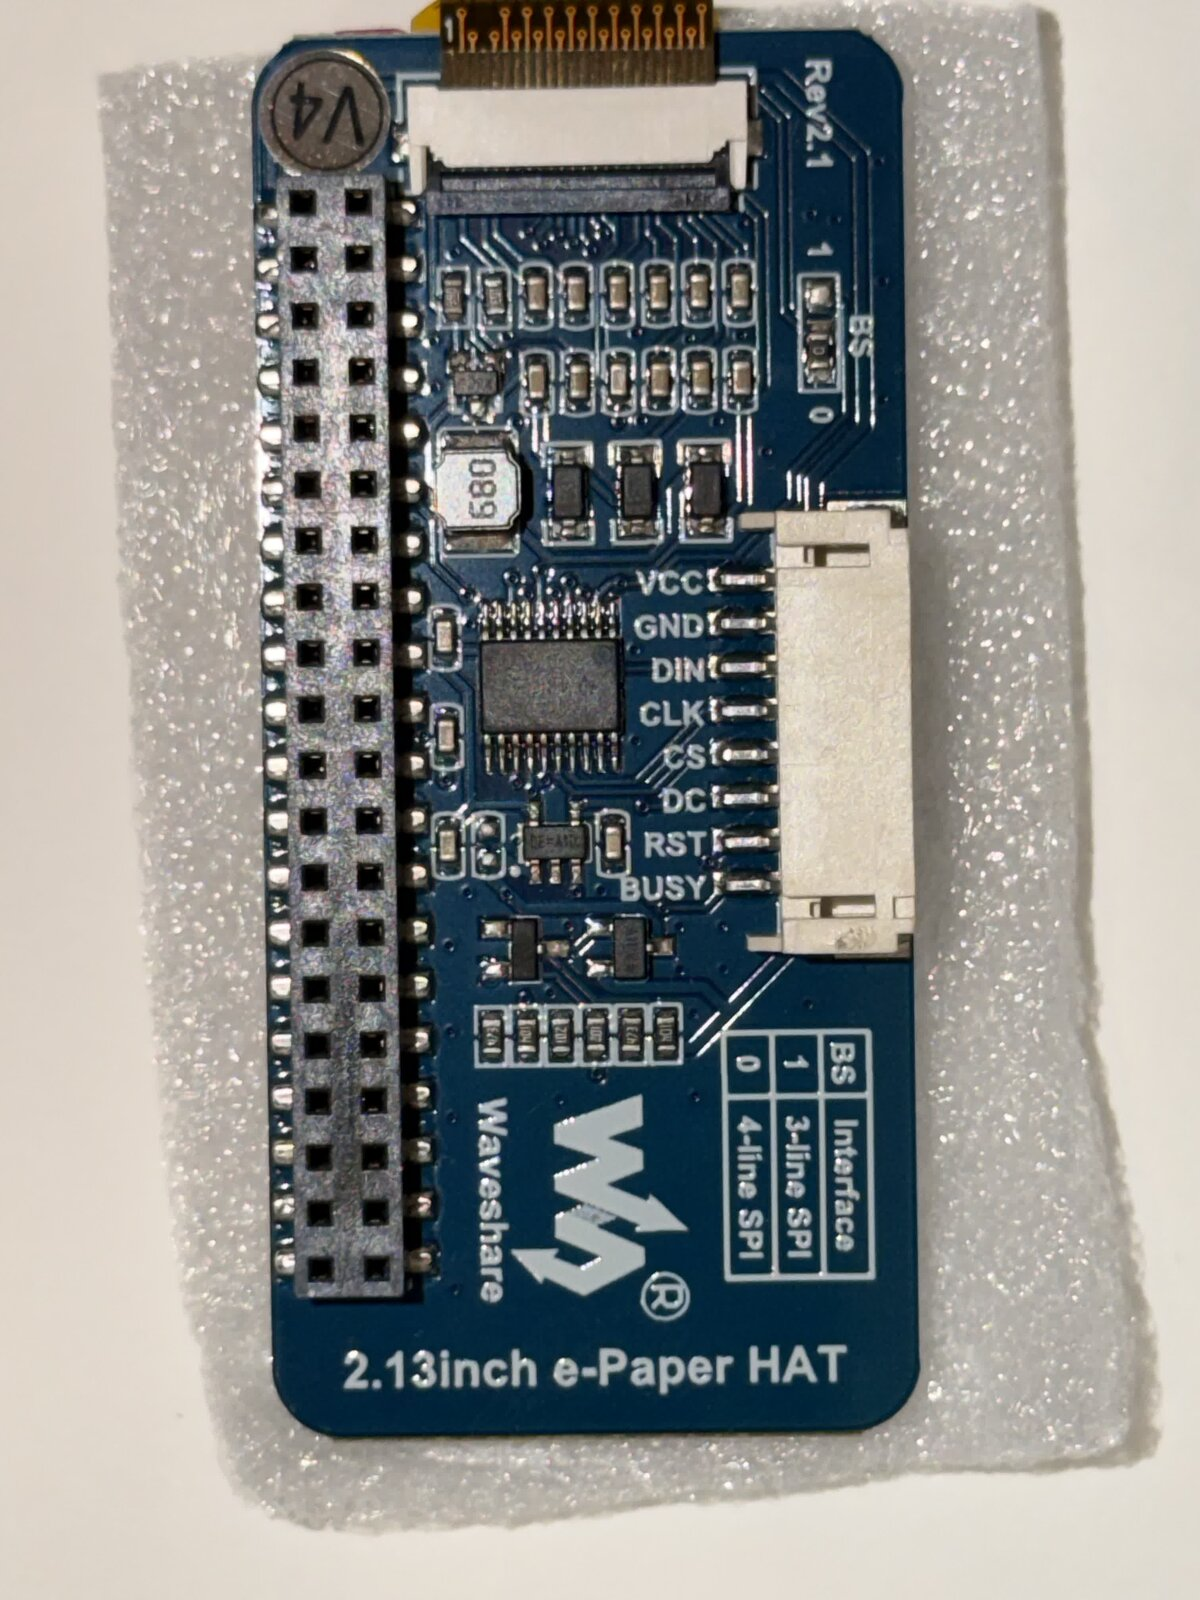
\includegraphics[height=0.66\textheight]{epaper-hat-back.jpg}
    \end{column}
    \begin{column}{0.36\textwidth}
      \begin{itemize}
        \item Zestaw nRF52 DK, e-papier, akcelerometr i odbiornik DCF-77 na płytce stykowej.
        \item Docelowo: lutowana płytka uniwersalna.
      \end{itemize}
    \end{column}
  \end{columns}
\end{frame}

%% 6. Niski pobór prądu
\begin{frame}{Jak oszczędzać energię}
  \begin{itemize}
    \item Procesor śpi cały czas; budzą go tylko przerwania: przyciski, akcelerometr, zegar RTC.
    \item Odbiornik DCF-77 jest włączony tylko w krótkim oknie synchronizacji.
    \item E-papier pobiera prąd wyłącznie podczas odświeżania.
  \end{itemize}
\end{frame}

%% 7. DCF-77
\begin{frame}{Synchronizacja czasu: DCF-77}
  \begin{itemize}
    \item Nadajnik we Frankfurcie, 77,5 kHz; jedna ramka na minutę zawiera pełny czas i datę.
    \item Bit to impuls 100 ms (zero) lub 200 ms (jeden) na początku sekundy.
    \item Okno synchronizacji o 03:00, a po niepowodzeniu ponowienia. Ramka ze złą parzystością jest odrzucana.
  \end{itemize}
\end{frame}

%% 8. Własny generator DCF-77
\begin{frame}{Własny generator DCF-77}
  \begin{columns}[c]
    \begin{column}{0.58\textwidth}
      \begin{itemize}
        \item W pomieszczeniu nie udało się odebrać prawdziwego sygnału, więc nie było czym testować dekodera.
        \item Płytka Nucleo-F411RE generuje ramkę czasu, także z celowymi błędami.
        \item Sztuczka: jedna nóżka generuje nośną 77,5 kHz, a w czasie impulsu zmieniamy jej wypełnienie. Amplituda spada do ok.\ 15\,\%, czyli powstaje prawdziwa modulacja. Sygnał trafia do anteny odbiornika przez pętlę obok niej.
      \end{itemize}
    \end{column}
    \begin{column}{0.40\textwidth}
      \centering
      %% źródło: temp-resources, moduł DCF-1060N z anteną ferrytową
      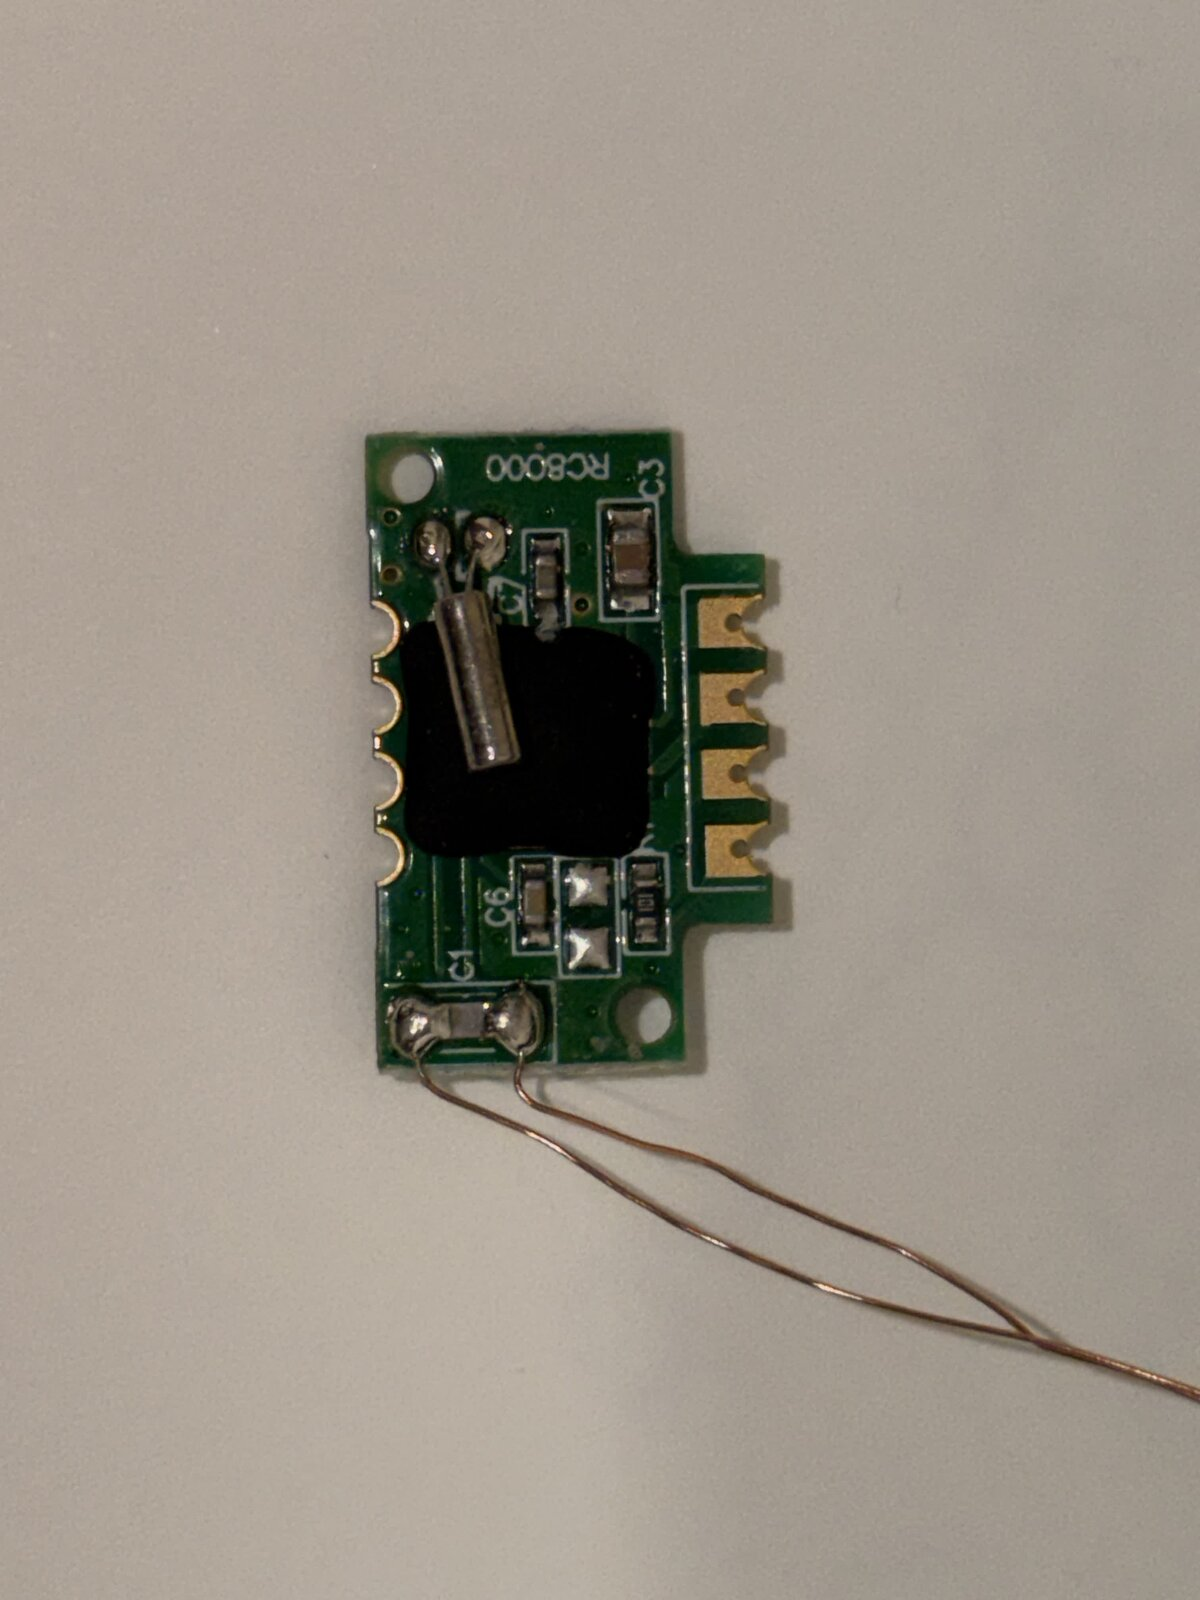
\includegraphics[width=\textwidth]{dcf77-module.jpg}
    \end{column}
  \end{columns}
\end{frame}

%% 9. Wyświetlacz i wyłączanie ruchem
\begin{frame}{Wyświetlacz i wyłączanie ruchem}
  \begin{columns}[c]
    \begin{column}{0.30\textwidth}
      \centering
      %% źródło: temp-resources, tarcza zegara na e-papierze (zdjęcie z telefonu)
      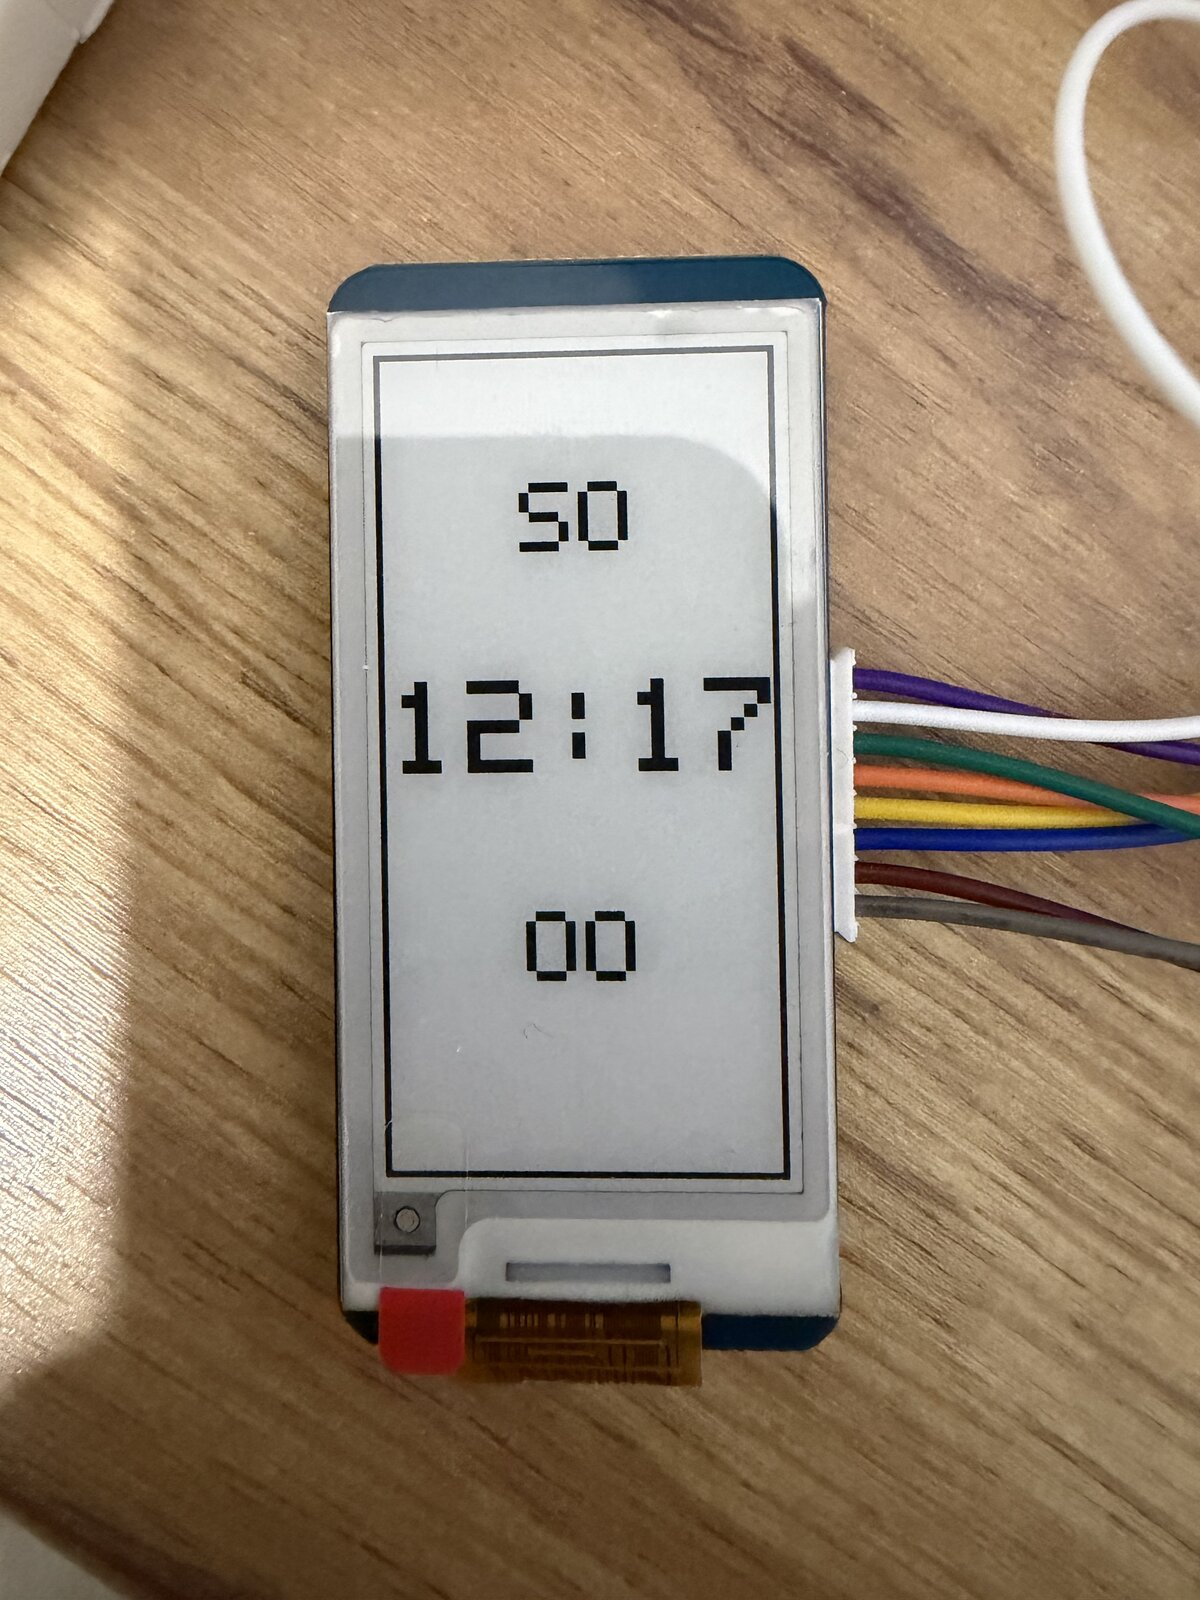
\includegraphics[height=0.72\textheight]{clock-face-upright.jpg}
    \end{column}
    \begin{column}{0.66\textwidth}
      \begin{itemize}
        \item Tarcza: godzina, dzień tygodnia, stan alarmu; własne glify, bez zewnętrznej biblioteki grafiki.
        \item Alarm cichnie po 20 zdarzeniach z akcelerometru (przerwanie INT1) w ciągu 30 s. Każdy przycisk wycisza od razu.
      \end{itemize}
    \end{column}
  \end{columns}
\end{frame}

%% 10. Pomiary
\begin{frame}{Pomiary prądu (PPK2)}
  \centering
  %% źródło: notes/measurements/ppk-20261025T210658.ppkz, okno 380-545 s; notatka notes/log/2026-10-24_deep-sleep-current.md, seria C5
  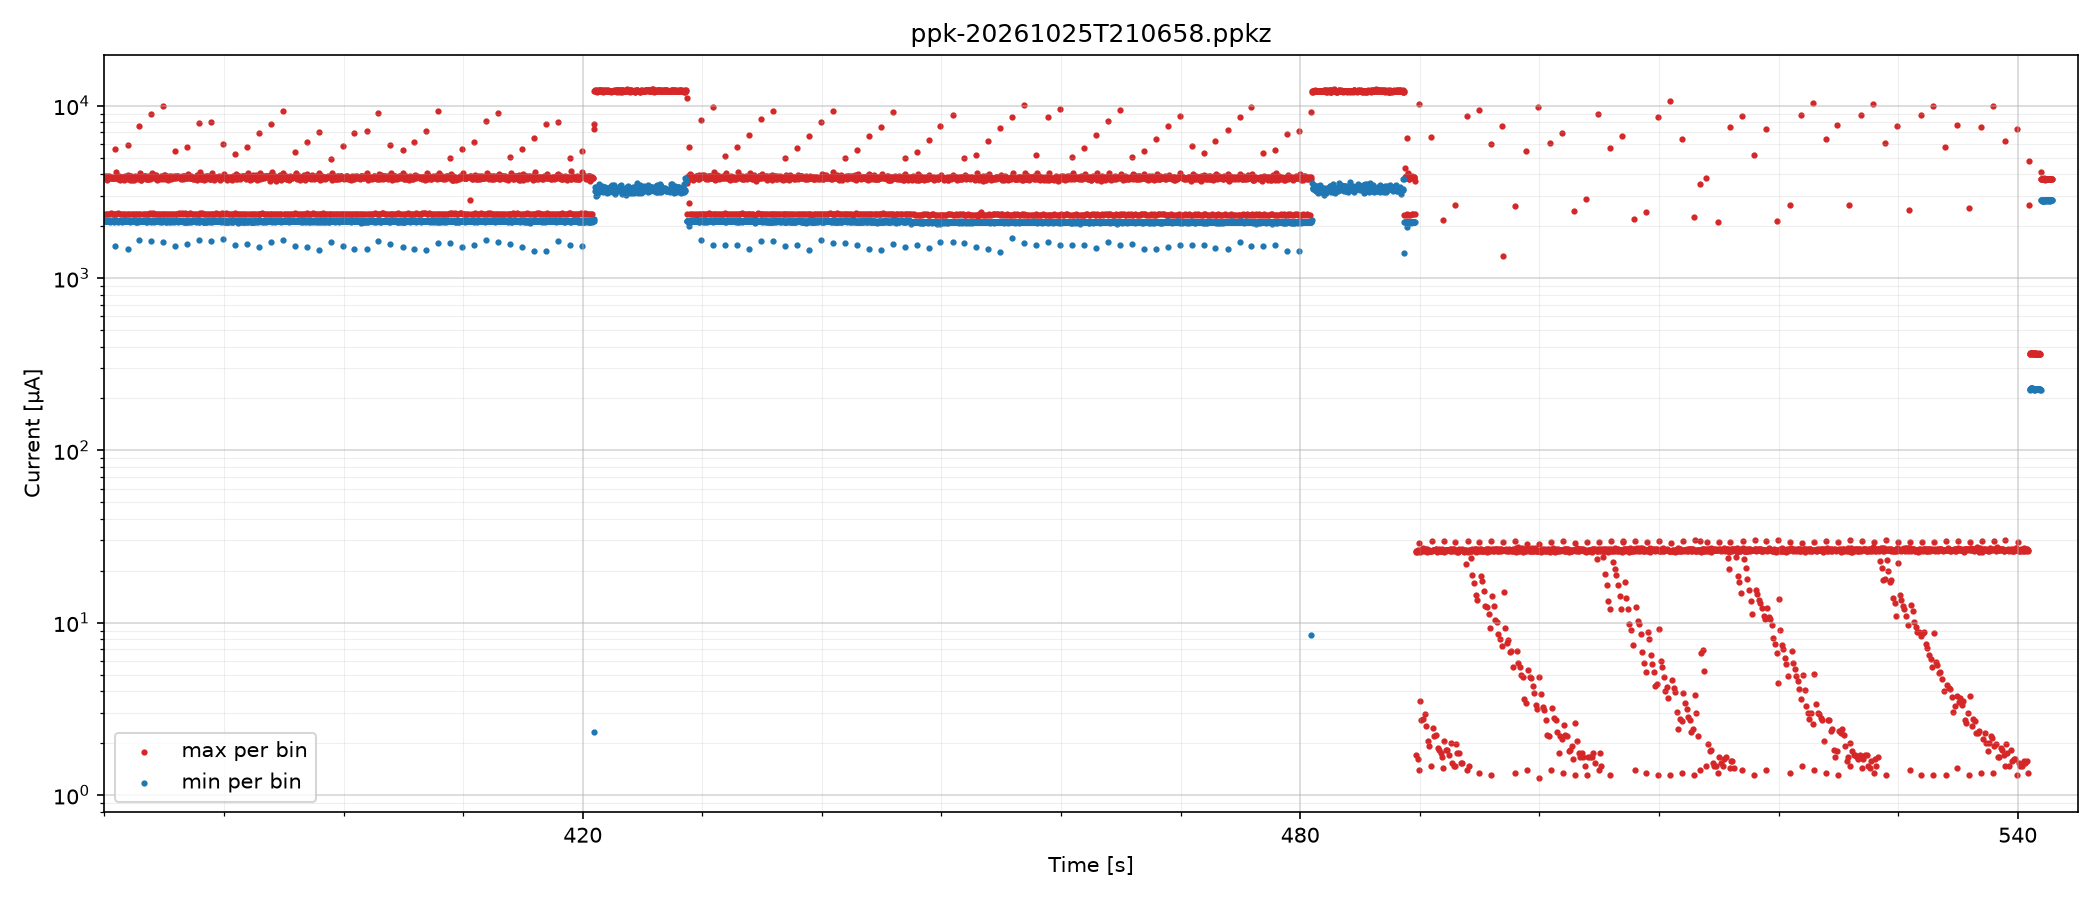
\includegraphics[width=0.78\textwidth]{ppk2-epd-rst.png}
  \begin{itemize}
    \item Seria C5: w spoczynku 2,06 mA. Po odłączeniu jednego przewodu (\texttt{EPD\_RST}) spada do ok.\ 2\,\textmu A.
    \item Winowajca: firmware trzymał wysoki stan na wejściu RST wyświetlacza.
  \end{itemize}
\end{frame}

%% 11. Status i kierunek
\begin{frame}{Gdzie jestem i dokąd idę}
  \begin{itemize}
    \item \textbf{Jest:} działający zegar na e-papierze, synchronizacja DCF-77, wyłączanie alarmu ruchem, uśpienie procesora.
    \item \textbf{Dalej:} dokończyć pomiary energii, dodać konfigurację przez Bluetooth i stronę WWW, napisać pracę.
  \end{itemize}
  \vfill
  \small stan na 27.10.2026
\end{frame}

\end{document}
